% Plane partition
% Author: Jang Soo Kim
%\documentclass{minimal}
%\usepackage{tikz}
% Three counters
\newcounter{x}
\newcounter{y}
\newcounter{z}

% The angles of x,y,z-axes
\newcommand\xaxis{210}
\newcommand\yaxis{-30}
\newcommand\zaxis{90}

% The top side of a cube
\newcommand\topside[3]{
  \fill[fill=yellow, draw=black,shift={(\xaxis:#1)},shift={(\yaxis:#2)},
  shift={(\zaxis:#3)}] (0,0) -- (30:1) -- (0,1) --(150:1)--(0,0);
}

% The left side of a cube
\newcommand\leftside[3]{
  \fill[fill=red, draw=black,shift={(\xaxis:#1)},shift={(\yaxis:#2)},
  shift={(\zaxis:#3)}] (0,0) -- (0,-1) -- (210:1) --(150:1)--(0,0);
}

% The right side of a cube
\newcommand\rightside[3]{
  \fill[fill=blue, draw=black,shift={(\xaxis:#1)},shift={(\yaxis:#2)},
  shift={(\zaxis:#3)}] (0,0) -- (30:1) -- (-30:1) --(0,-1)--(0,0);
}

% The cube 
\newcommand\cube[3]{
  \topside{#1}{#2}{#3} \leftside{#1}{#2}{#3} \rightside{#1}{#2}{#3}
}

% Definition of \planepartition
% To draw the following plane partition, just write \planepartition{ {a, b, c}, {d,e} }.
%  a b c
%  d e
\newcommand\planepartition[1]{
 \setcounter{x}{-1}
  \foreach \a in {#1} {
    \addtocounter{x}{1}
    \setcounter{y}{-1}
    \foreach \b in \a {
      \addtocounter{y}{1}
      \setcounter{z}{-1}
      \foreach \c in {1,...,\b} {
        \addtocounter{z}{1}
        \cube{\value{x}}{\value{y}}{\value{z}}
      }
    }
  }
}

%\begin{document} 

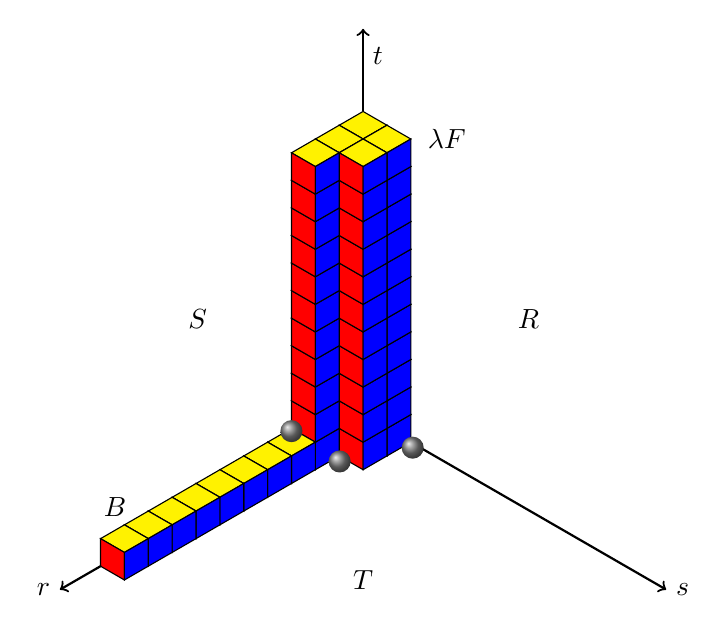
\begin{tikzpicture}[scale=0.35]



\newcommand{\redbox}[3]{ 
\draw[fill=red, draw=black,shift={(\xaxis:#1)},shift={(\yaxis:#2)},shift={(\zaxis:#3)}]
(0,0) rectangle (1,1);
}
\newcommand{\yellowbox}[3]{ 
\draw[fill=yellow, draw=black,shift={(\xaxis:#1)},shift={(\yaxis:#2)},shift={(\zaxis:#3)}]
(0,0) rectangle (1,1);
}
\newcommand{\bluebox}[3]{ 
\draw[fill=blue, draw=black,shift={(\xaxis:#1)},shift={(\yaxis:#2)},shift={(\zaxis:#3)}]
(0,0) rectangle (1,1);
}




\planepartition{{11,11},{11,11},{11},{1},{1},{1},{1},{1},{1},{1},{1}}

\draw [thick,->] (0,11)-- (0,14);
\draw [thick,->] (1.74,-1.74*0.57735)-- (11,-11*0.57735);
\draw [thick,->]  (-9.5,-9.5*0.57735)-- (-11,-11*0.57735);

\node [right] at (0,13) {$t$};
\node [right] at (11,-11*0.57735) {$s$};
\node [left] at  (-11,-11*0.57735) {$r$};
\node [above] at  (-9,-7*0.57735) {$B$};
\node [right] at (2,10) {$\lambda F$};
\node  at (6,6*0.57735) {$R$};
\node  at (-6,6*0.57735) {$S$};
\node  at (0,-6) {$T$};

\shade [ball color=gray] (-2.6,-.6) circle [radius=0.4cm];
\shade [ball color=gray] (1.8,-1.2) circle [radius=0.4cm];
\shade [ball color=gray] (-0.85,-1.7) circle [radius=0.4cm];


\end{tikzpicture}

%\end{document} 
